\chapter{Tredicesima lezione (24/11/2015)}

\section{Limite di funzione (cont.)}

Analogamente a quanto fatto per le successioni, vediamo ora il teorema del confronto applicato alle funzioni.
\begin{theorem}[\bfseries Teorema del confronto]
Siano $f, g, h$ funzioni definite da $A \to \R$. Se:
\begin{itemize}
\item $f(x) \le g(x) \le h(x)$ per ogni $x \in A \backslash\{x_0\}$
\item $\lim_{x \to x_0} f(x) = \lim_{x \to x_0} h(x) = L$
\end{itemize}
Allora 
\begin{equation*}
\lim_{x \to x_0} g(x) = L
\end{equation*}
\end{theorem}

\begin{proof}
Per definizione di limite, $\forall \epsilon > 0$ esiste un intorno $B'_{\delta_1} (x_0)$ tale che $\forall x \in B'_{\delta_1} (x_0)$ vale $L-\epsilon < f(x) < L + \epsilon$. Stiamo quindi dicendo che se $0 < |x - x_0| < \delta_1$ allora $|f(x)-L| < \epsilon$.

Per lo stesso ragionamento esiste $\delta_2$ tale che se $x \in B'_{\delta_2} (x_0)$ allora $L-\epsilon < h(x) < L + \epsilon$.

Scegliamo $\delta = \min\{\delta_1, \delta_2\}$: se ora $x$ appartiene all'intorno $B'_\delta (x_0)$ allora vale
\begin{gather*}
L-\epsilon < f(x) \le g(x) \le h(x) < L + \epsilon \\
L-\epsilon \le g(x) \le L + \epsilon \\
\end{gather*}
Abbiamo quindi fatto vedere che $\lim_{x \to x_0} g(x) = L$.
\end{proof}

\begin{example}
Vogliamo calcolare
\begin{equation*}
\lim_{x \to 0} \left\lvert x \cdot \sin \frac{1}{x} \right\rvert
\end{equation*}
È semplice osservare che $0 \le |x \cdot \sin \frac{1}{x}| \le |x|$. Poiché il limite per $x \to 0$ della prima e della terza funzione è evidentemente zero, allora anche il limite cercato vale zero per il teorema del confronto.
\end{example}

\begin{proposition}
Sia $A$ un intervallo aperto e la funzione $f : A \to \R$ non decrescente (e limitata inferiormente). Dato $x_0 \in A$:
\begin{itemize}
\item $\lim_{x \to x_0^+} f(x) = \inf \set{f(x) | x \in A, x > x_0}$
\item $\lim_{x \to x_0^-} f(x) = \inf \set{f(x) | x \in A, x < x_0}$
\end{itemize}
\end{proposition}

Dimostriamo il primo punto, poiché il secondo è analogo.
\begin{proof}
L'insieme $\set{f(x) | x \in A, x > x_0}$ è inferiormente limitato e quindi ha un $\inf \set{f(x) | x \in A, x > x_0} = L$.

Per ogni $\epsilon > 0$ esiste un $y > x_0$ con $f(x) < L + \epsilon$. Essendo $f$ non decrescente, se $x \le y$ allora $f(x) \le f(y) < L + \epsilon$.

Osserviamo anche che $L \le f(x)$ perché $L$ è un minorante. Quindi $\forall \epsilon$ esiste $y$ tale che
\begin{equation*}
x_0 < x < y \implies L - \epsilon < f(x) < L + \epsilon
\end{equation*}
ovvero $\lim_{x \to x_0^+} f(x) = L$.
\end{proof}

Questa proposizione vale comunque per $f(x_0, b) \to \R$ limitata inferiormente e non decrescente, vale infatti lo stesso ragionamento.

\begin{definition}
Sia data una funzione $f: A \to \R$ definita sull'intervallo aperto $A$ e $x_0 \in A$. Si dice che $\lim_{x \to x_0} f(x) = +\infty$ se per ogni $M > 0$ esiste $\delta > 0$ tale che $\forall x \in B'_\delta (x_0)$ vale $f(x) > M$.
\end{definition}

Si dice che $(M, +\infty)$ è un intorno di $+\infty$. La definizione quindi dice che $\lim_{x \to x_0} f(x) = +\infty$ se per ogni intorno $U$ di $+\infty$ esiste $\delta > 0$ tale che $x_0 \in B'_\delta (x_0) \implies f(x) \in U$.

Analoga definizione vale per gli intorni di $-\infty$, che sono del tipo $(-\infty, -M)$.

\begin{example}
Mostriamo, come è facilmente deducibile dal grafico della funzione logaritmo, che
\begin{equation*}
\lim_{x \to 0^+} \log x = -\infty
\end{equation*}
Per ogni $M > 0$ esiste $\delta > 0$ tale che se $0 < x < \delta$ allora $\log x < -M$. Ciò significa che $x < e^{-M}$: possiamo porre $\delta = e^{-M}$ per far sì che la condizione sia verificata.
\end{example}

\begin{definition}
Dato un intervallo $A = (a, +\infty)$ e una funzione $f: A \to R$ diciamo che
\begin{equation*}
\lim_{x \to +\infty} f(x) = L
\end{equation*}
se per ogni intorno $U$ di $L$ esiste $M$ tale che per $x > M \implies f(x) \in U$.
\end{definition}

\begin{theorem}
Sia data una funzione $f: A \to \R$ definita sull'intervallo $A = (a, +\infty)$. 

\begin{itemize}
\item $\lim_{x \to +\infty} f(x) = L$ se e solo se per ogni successione $\{x_n\}$ in $A$ divergente a $+\infty$, vale $\lim_{n \to +\infty} f(x_n) = L$.

\item $\lim_{x \to +\infty} f(x) = +\infty$ se e solo se per ogni successione $\{x_n\}$ in $A$ divergente a $+\infty$, vale $\lim_{n \to +\infty} f(x_n) = +\infty$.

\item $\lim_{x \to x_0} f(x) = +\infty$ se e solo se per ogni successione $\{x_n\}$ in $A \backslash\{x_0\}$ convergente a $x_0$, vale $\lim_{n \to +\infty} f(x_n) = +\infty$.

\end{itemize}
\end{theorem}

\begin{example}
Riprendendo l'esempio precedente sul calcolo di $\lim \log x$:  consideriamo una successione infinitesima positiva $\{\epsilon_n\}$. Avevamo già visto che $\lim \log (\epsilon_n) = -\infty$. Grazie al teorema sappiamo che questo vale anche per la funzione.
\end{example}

\section{Funzioni continue}
\begin{definition}
Una funzione $f: A \to \R$ è \emph{continua in $x_0 \in A$} se per ogni intorno $V$ di $f(x_0)$ esiste $\delta > 0$ tale che per ogni $x \in B_\delta (x_0)$ vale $f(x) \in V$.
\end{definition}

Osserviamo che la definizione è simile a quella di limite, con la differenza che ora stiamo considerando l'intorno $B_\delta (x_0)$ che include il punto $x_0$.

\begin{definition}
Una funzione è \emph{continua} se è continua in ogni $x \in A$ (dove $A$ è il dominio della funzione).
\end{definition}

\begin{proposition}
Dato un intervallo aperto $A$, $f: A \to \R$ è continua in $x_0 \in A$ se e solo se
\begin{equation*}
\lim_{x \to x_0} f(x) = f(x_0)
\end{equation*}
\end{proposition}

\begin{proof}
Sia $f$ una funzione continua in $x_0$; allora per ogni intorno $V$ di $f(x_0)$ $\exists \delta$ tale che $x \in B'_\delta (x_0) \implies f(x) \in V$. L'affermazione è vera perché abbiamo solo tolto il punto $x_0$ dall'intorno. Quindi
\begin{equation*}
\lim_{x \to x_0} f(x) = f(x_0)
\end{equation*}
\end{proof}

Dimostriamo il viceversa.
\begin{proof}
Sia $\lim_{x \to x_0} f(x) = f(x_0)$. Per definizione di limite per ogni intorno $V$ di $f(x_0)$ $\exists \delta$ tale che $0 < |x - x_0| < \delta \implies f(x) \in V$. Se $x = x_0$ allora $f(x_0) \in V$, quindi $|x-x_0| < \delta \implies f(x) \in V$.
\end{proof}

\begin{example}
La funzione $f(x) = x$ è continua, perché $\lim_{x \to x_0} x = x_0$.
\end{example}

\begin{example}
La funzione $f(x) = \sin x$ è continua. Per dimostrarlo, occorre ragionare con le formule di prostaferesi. Ricordiamo che:
\begin{align*}
\sin(\alpha + \beta) - \sin (\alpha - \beta) &= \sin \alpha \cos \beta + \cos \alpha \sin \beta - \sin \alpha \cos \beta + \cos \alpha \sin \beta \\
&= 2\cos \alpha \sin \beta
\end{align*}

Ci serve far vedere che
\begin{equation*}
\lim_{x \to x_0} \sin x = \sin x_0
\end{equation*}
cioè che 
\begin{equation*}
\lim_{h \to 0} \sin(x_0 + h) = \sin (x_0)
\end{equation*}

Se poniamo $\alpha = x_0 + \frac{h}{2}$ e $\beta = \frac{h}{2}$ allora
\begin{equation*}
\sin (x_0 + h) - \sin x_0 = 2 \cos \left(x_0 + \frac{h}{2}\right) \cdot \sin \left(\frac{h}{2}\right)
\end{equation*}

Quindi, usando il fatto che $0 \le |\cos x| \le 1$:
\begin{equation*}
|\sin(x_0+h)-\sin x_0| \le 2\left\lvert \sin \frac{h}{2} \right\rvert \le 2 \left\lvert\frac{h}{2}\right\rvert= |h|
\end{equation*}

Quindi, essendo $\lim_{x \to 0} |h| = 0$, usando il teorema del confronto si ha che
\begin{equation*}
\lim |\sin(x_0+h)-\sin x_0| = 0
\end{equation*}
Se il limite è zero in valore assoluto, allora lo è anche senza. Quindi abbiamo fatto vedere che $\sin x$ è continua.
\end{example}

\begin{example}
La funzione $f(x) = e^x$ è continua. Infatti $e^x = e^{x_0} \cdot e^{x-x_0}$, quindi
\begin{equation*}
\lim_{x \to x_0} e^x = e^{x_0} \iff \lim_{x \to x_0} e^{x_0} \cdot (e^{x-x_0}) = e^{x_0} \iff \lim_{x \to x_0} e^{x-x_0} = 1
\end{equation*}
Ci dobbiamo chiedere quindi se $\lim_{x \to 0} e^x = 1$. Studiamo separatamente il limite destro e il limite sinistro.

Affinché $\lim_{x \to 0^+} e^x = 1$ basta $\lim_{n \to +\infty} e^{\frac{1}{n}} = 1$ perché dato $\epsilon$ esiste $n$ tale che
\begin{equation*}
e^\frac{1}{n} < 1 + \epsilon \implies \forall x < \frac{1}{n} \quad e^x < 1 + \epsilon
\end{equation*}

Quindi $e^\frac{1}{n} < 1 + \epsilon \iff e < (1+\epsilon)^n$, che è vero definitivamente. Quindi $\lim_{n \to +\infty} e^\frac{1}{n} = 1$ e quindi $\lim_{x \to 0^+} e^x = 1$.

Per il limite da sinistra dobbiamo verificare invece che
\begin{equation*}
\lim_{n \to +\infty} e^{-\frac{1}{n}} = 1
\end{equation*}
Cioè $\forall \epsilon > 0$ vale definitivamente che 
\begin{align*}
e^{-\frac{1}{n}} &> 1 - \epsilon\\
\frac{1}{\epsilon} &> (1 - \epsilon)^n \\
e &< \frac{1}{(1-\epsilon)^n}
\end{align*}
Quindi il limite $\lim_{n \to +\infty} e^{-\frac{1}{n}} = 1$: $\forall \epsilon \; \exists N$ tale che $e^{-\frac{1}{n}} > 1 - \epsilon$.
Se $-\frac{1}{n} < x < 0$ allora
\begin{equation*}
1 - \epsilon < e^{-\frac{1}{n}} < e^x < 1
\end{equation*}
Quindi anche $\lim_{x \to 0^-} e^x = 1$.
\end{example}

\begin{proposition}
Siano $f, g: A \to \R$ funzioni continue. Allora:
\begin{itemize}
\item $f + g$ e $f \cdot g$ sono funzioni continue
\item se $g \neq 0$ in ogni punto di $A$, la funzione $\frac{f}{g}$ è continua
\end{itemize}
\end{proposition}
\begin{proof}
La dimostrazione è banale e si fa usando l'algebra dei limiti. Dimostriamo a titolo di esempio la continuità della somma di funzioni continue. Dato $x_0 \in A$ deve valere affinché ci sia la continuità:
\begin{equation*}
\lim_{x \to x_0} (f(x)+g(x)) = f(x_0) + g(x_0)
\end{equation*}
Questo è ovvio, perché
\begin{equation*}
\lim_{x \to x_0} (f(x)+g(x)) = \lim_{x \to x_0} f(x) + \lim_{x \to x_0} g(x) = f(x_0) + g(x_0)
\end{equation*}
\end{proof}

\begin{remark}
Grazie a quanto abbiamo affermato e dimostrato, possiamo dire che tutti i polinomi sono funzioni continue. Infatti, essi sono ottenuti dal prodotto e dalla somma di funzioni continue (ad esempio $x^2 = x \cdot x$ e così via).
\end{remark}

Inoltre ora siamo anche in grado di calcolare direttamente alcuni limiti.
\begin{example}
\begin{equation*}
\lim_{x \to 2} \frac{x^2 + 3x}{x - 3} = \frac{2^2 + 3 \cdot 2}{2 - 3} = -10
\end{equation*}
\end{example}

\section{Punti di discontinuità}
Sia data una funzione $f: A \to R$ (dove $A$ è sempre un intervallo aperto) e un punto $x_0 \in A$.

\begin{itemize}
\item Si dice che la funzione ha una \emph{discontinuità di prima specie} in $x_0$ se i limiti destro e sinistro esistono (finiti) e sono diversi.
\item Si dice che la funzione ha una \emph{discontinuità di seconda specie} in $x_0$ se almeno uno tra il limite destro e sinistro è infinito oppure non esiste.
\item Si dice che la funzione ha una \emph{discontinuità eliminabile} in $x_0$ se il limite $\lim_{x \to x_0} f(x)$ esiste (finito) ma è diverso dal valore $f(x_0)$.
\end{itemize}

\begin{example}
Consideriamo la funzione ``parte intera di $x$'': $f(x) = [x]$, il cui grafico è il seguente.
\begin{center}
\begin{tikzpicture}[scale=0.5]
\draw[->] (-2.5,0) -- (3.2,0) node[right] {$x$};
\draw[->] (0,-2.5) -- (0,2.2) node[above] {$y$};
\draw [line width=2pt, domain=0:1] plot (\x, 0);
\draw [line width=2pt, domain=1:2] plot (\x, 1);
\draw [line width=2pt, domain=2:3] plot (\x, 2);
\draw [line width=2pt, domain=-1:0] plot (\x, -1);
\draw [line width=2pt, domain=-2:-1] plot (\x, -2);
\end{tikzpicture}
\end{center}
La funzione è continua in ogni $x \notin \Z$; nei punti $x \in \Z$ la funzione ha una discontinuità di prima specie.
\end{example}

\begin{example}
Consideriamo una funzione così definita:
\begin{equation*}
f(x) = \begin{cases}
\log |x| & x \neq 0 \\
0 & x = 0
\end{cases}
\end{equation*}
\begin{center}
\begin{tikzpicture}[scale=0.5]
\draw[->] (-2.5,0) -- (3.2,0) node[right] {$x$};
\draw[->] (0,-2.5) -- (0,2.2) node[above] {$y$};
\draw [domain=0.1:3] plot (\x, ln{\x});
\draw [domain=-3:-0.1] plot (\x, ln{-\x});
\draw [line width=2pt, domain=-0.1:0.1] plot (\x, 0);
\end{tikzpicture}
\end{center}
In 0 la funzione presenta una punto di discontinuità di seconda specie.
\end{example}

\begin{example}
Consideriamo una funzione così definita:
\begin{equation*}
f(x) = \begin{cases}
x \cdot \sin \frac{1}{x} & x \neq 0 \\
1 & x = 0
\end{cases}
\end{equation*}
\begin{center}
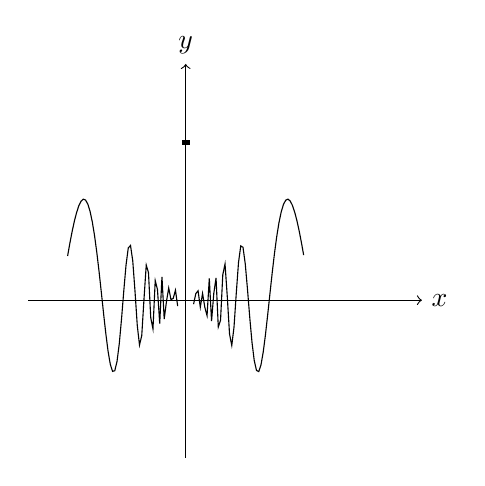
\begin{tikzpicture}[scale=10]
\draw[->] (-0.2,0) -- (0.3,0) node[right] {$x$};
\draw[->] (0,-0.2) -- (0,0.3) node[above] {$y$};
\draw [domain=0.01:0.15,samples=50] plot (\x, {\x*sin((1/\x)r)});
\draw [domain=-0.15:-0.01,samples=50] plot (\x, {\x*sin((1/\x)r)});
\draw [line width=2pt, domain=-0.005:0.005] plot (\x, 0.2);
\end{tikzpicture}
\end{center}
In 0 $\lim_{x \to 0} f(x) = 0$, quindi la funzione presenta una punto di discontinuità eliminabile (in questo caso semplicemente definendo la funzione come $f(0) = 0$).
\end{example}


\begin{example}
Consideriamo la funzione
\begin{equation*}
f(x) = \sin \frac{1}{x}
\end{equation*}
\begin{center}
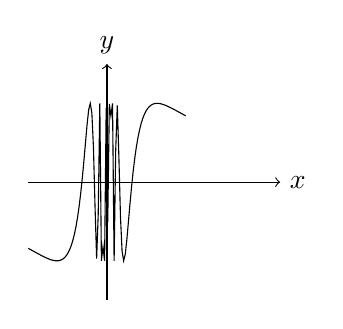
\begin{tikzpicture}[scale=1]
\draw[->] (-1,0) -- (2.2,0) node[right] {$x$};
\draw[->] (0,-1.5) -- (0,1.5) node[above] {$y$};
\draw [domain=0.01:1,samples=50] plot (\x, {sin((1/\x)r)});
\draw [domain=-1:-0.01,samples=50] plot (\x, {sin((1/\x)r)});
\end{tikzpicture}
\end{center}
In 0 la funzione presenta una discontinuità di seconda specie perché lì $\nexists \lim_{x \to 0} \sin \frac{1}{x}$.
\end{example}

In generale, una funzione $f: A \to \R$ si dice continua in $x_0$ se per ogni intorno $U$ di $f(x_0)$ $\exists \delta > 0$ tale che
\begin{equation*}
x \in B_\delta (x_0) \cap A \implies f(x) \in V
\end{equation*}
Se consideriamo $A = [a, b]$, la funzione $f:A \to \R$ è continua in $a$ se e solo se
\begin{equation*}
\lim_{x \to a^+} f(x) = f(a)
\end{equation*}

\section{Funzioni continue e successioni}
Enunciamo ora formalmente un teorema che abbiamo già usato diverse volte nella risoluzione delle successioni.

\begin{theorem}
Sia $f: [a, b] \to \R$ una funzione continua e $\{x_n\}$ una successione in $[a, b]$ che converge a $L$. Allora
\begin{equation*}
\lim_{n \to +\infty} f(x_n) = f(L)
\end{equation*}
\end{theorem}

\begin{example}
\begin{equation*}
\lim_{n \to +\infty} e^\frac{n}{n + 1} = e
\end{equation*}
perché $\lim \frac{n}{n+1} = 1$ e $f(x) = e^x$ è una funzione continua.
\end{example}

\begin{proof}
Osserviamo subito che $L \in [a, b]$. Infatti, se fosse $L > b$ per la permanenza del segno avremmo che $x_n - b > 0$ definitivamente; e questo è assurdo perché $x_n < b$. Quindi $f(L)$ è ben definito, perché $L$ appartiene al dominio della funzione.

Preso $U$, intorno di $f(L)$, per definizione di continuità in $L$ esiste $\delta$ tale che
\begin{equation*}
x \in B_\delta (L) \implies f(x) \in U
\end{equation*}
Poiché $x_n$ è definitivamente appartenente a $B_\delta (L)$, allora definitivamente $f(x_n) \in U$. Quindi
\begin{equation*}
\lim_{n \to +\infty} f(x_n) = f(L)
\end{equation*}
\end{proof}